\documentclass[aspectratio=169]{beamer}
\usepackage[english]{babel}
\usepackage[fntef]{ctex} % invole CJKfntef
\usepackage{hyperref}
\usepackage{ctex}
\usepackage{amsthm}
\usepackage{mathtools}
\usepackage{bm}
\usepackage{physics}
\usepackage{calligra}
\usepackage{csquotes}
\usepackage{tensor}
\usepackage[thicklines]{cancel}
\usepackage{tcolorbox}
\usepackage{pstricks}
\usepackage{graphicx}
\usepackage[backend=biber, bibstyle=nature, sorting=nty, citestyle=numeric-comp]{biblatex} %Custom bibliography
    \addbibresource{bib.bib} %Load references


\DeclareMathAlphabet{\mathcalligra}{T1}{calligra}{m}{n}
\DeclareFontShape{T1}{calligra}{m}{n}{<->s*[2.2]callig15}{}
\newcommand{\scriptr}{\mathcalligra{r}\,}
\newcommand{\boldscriptr}{\pmb{\mathcalligra{r}}\,}
\def\rc{\scriptr}
\def\brc{\boldscriptr}
\def\hrc{\hat\brc}
\newcommand{\ie}{\emph{i.e.}} %id est
\newcommand{\eg}{\emph{e.g.}} %exempli gratia
\newcommand{\rtd}[1]{\ensuremath{\left\lfloor #1 \right\rfloor}}
\newcommand{\dirac}[1]{\ensuremath{\delta \left( #1 \right)}}
\newcommand{\diract}[1]{\ensuremath{\delta^3 \left( #1 \right)}}
\newcommand{\e}{\ensuremath{\epsilon_0}}
\newcommand{\m}{\ensuremath{\mu_0}}
\newcommand{\V}{\ensuremath{\mathcal{V}}}
\newcommand{\prnt}[1]{\ensuremath{\left(#1\right)}} %parentheses
\newcommand{\colch}[1]{\ensuremath{\left[#1\right]}} %square brackets
\newcommand{\chave}[1]{\ensuremath{\left\{#1\right\}}}  %curly brackets

\useoutertheme{infolines}
\useinnertheme{rectangles}
\usefonttheme{professionalfonts}


\definecolor{orange}{HTML}{1f4f94} %背景粉CC0099,蓝色1f4f94,绿色66CC33
\definecolor{gray}{HTML}{FFFFFF}	%底色白
\definecolor{yellow}{HTML}{6633FF}	%f0be52,红色FF0033 %\alert的颜色
\definecolor{lightorange}{HTML}{FF0033} %f19e58
\definecolor{textColor}{HTML}{000000} %黑

\renewcommand{\CancelColor}{\color{orange}}

\makeatletter
\newcommand{\mybox}[1]{%
  \setbox0=\hbox{#1}%
  \setlength{\@tempdima}{\dimexpr\wd0+13pt}%
  \begin{tcolorbox}[colback=orange,colframe=orange,boxrule=0.5pt,arc=4pt,
      left=6pt,right=6pt,top=6pt,bottom=6pt,boxsep=0pt,width=\@tempdima]
    \textcolor{white}{#1}
  \end{tcolorbox}
}
\makeatother

\usecolortheme[named=orange]{structure}
\usecolortheme{sidebartab}
\usecolortheme{orchid}
\usecolortheme{whale}
\setbeamercolor{alerted text}{fg=yellow}
\setbeamercolor{block title alerted}{bg=alerted text.fg!90!black}
\setbeamercolor{block title example}{bg=lightorange!60!black}
\setbeamercolor{background canvas}{bg=gray}
\setbeamercolor{normal text}{bg=gray,fg=textColor}
\setbeamertemplate{headline}
{}

\setbeamertemplate{footline}
        {
      \leavevmode%
      \hbox{%
      \begin{beamercolorbox}[wd=.5\paperwidth,ht=2.25ex,dp=1ex,center]{author in head/foot}%
        \usebeamerfont{author in head/foot}\insertshortauthor~~(\insertshortinstitute)
      \end{beamercolorbox}%
      \begin{beamercolorbox}[wd=.5\paperwidth,ht=2.25ex,dp=1ex,center]{date in head/foot}%
        \usebeamerfont{date in head/foot}\insertshortdate{}%\hspace*{2em}

    %#turning the next line into a comment, erases the frame numbers
        %\insertframenumber{} / \inserttotalframenumber\hspace*{2ex} 

      \end{beamercolorbox}}%
  
      \vskip0pt%
    }


\setbeamertemplate{blocks}[rectangle]
\setbeamercovered{dynamic}

\setbeamertemplate{section page}
{
	\begin{centering}
		\begin{beamercolorbox}[sep=27pt,center]{part title}
			\usebeamerfont{section title}\insertsection\par
			\usebeamerfont{subsection title}\insertsubsection\par
		\end{beamercolorbox}
	\end{centering}
}

%\setbeamertemplate{subsection page}
%{
%	\begin{centering}
%		\begin{beamercolorbox}[sep=12pt,center]{part title}
%			\usebeamerfont{subsection title}\insertsubsection\par
%		\end{beamercolorbox}
%	\end{centering}
%}

\newcommand{\hlight}[1]{\colorbox{violet!50}{#1}}
\newcommand{\hlighta}[1]{\colorbox{red!50}{#1}}
\title{组会报告} %->->->->-> Check hyperref title <-<-<-<-<-
\subtitle{论文复现: \href{https://ieeexplore.ieee.org/document/8306094}{On the Coexistence Between Full-Duplex and NOMA}}
\author[Yong YANG]{Yong YANG}
\institute[BUPT]{
	Beijing University of Posts and Telecommunications\\
	\url{https://bupt-yy.github.io/}
} 
\date{\today}

\begin{document}
	
	\frame{\titlepage}
	%\begin{frame}{目$\quad$次}
	%\tableofcontents   
    %\end{frame}

\begin{frame}{\textbf{{\LARGE{S}}YSTEM {\LARGE{M}}ODEL}}
	
	\begin{columns}
	\column{.35\textwidth}
	\begin{figure}
		\centering
		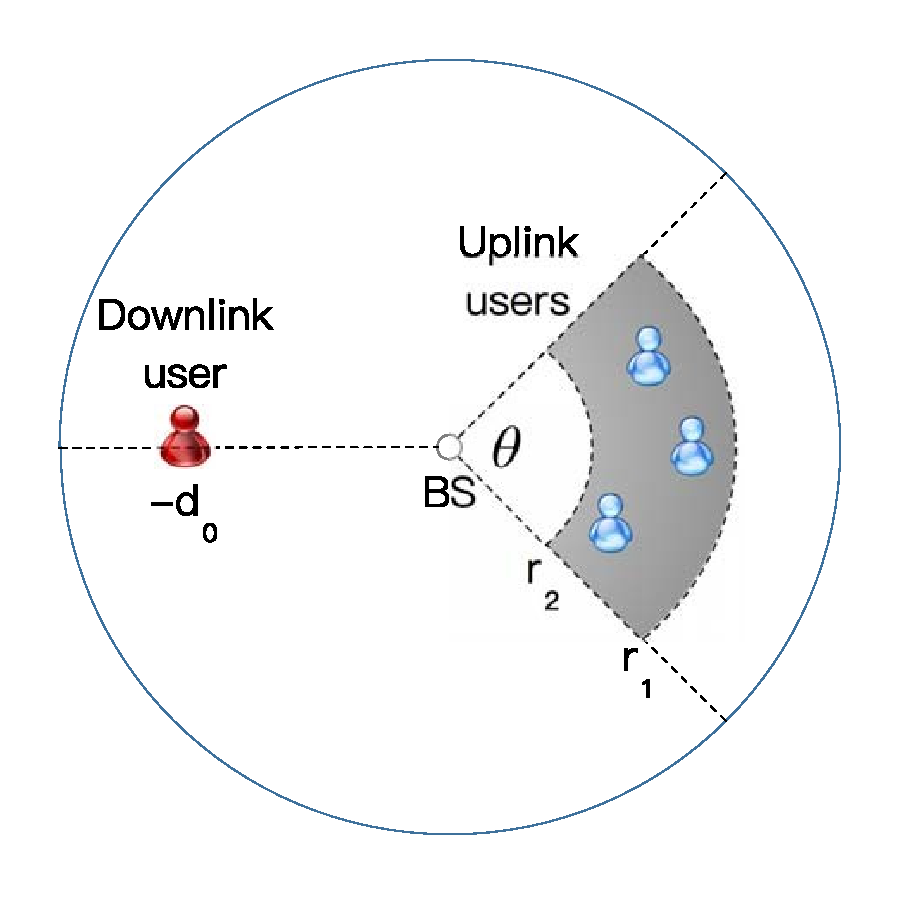
\includegraphics[width=1\linewidth]{images/fig1.pdf}
		\caption{1}
		\label{fig:fig1}
	\end{figure}
	
	\column{.65\textwidth}
	$1$个DL user位于$(-d_0,0)$, \\$M$个UL users均匀分布于$\mathrm{ann}(\text{BS},r_2,r_1;-\frac{\theta}{2},\frac{\theta}{2})$
	
	BS接收信号$y_{\text{BS}} = \sqrt{P_\text{U}}\sum_{m = 1}^{M}h_ms_m+h_{\text{SI}}\sqrt{P_{\text{SI}}}s_0+n_{\text{BS}}$.
	
	DL接收信号$y_{\text{D}}\,\, =  \sqrt{P_{\text{U}}}\sum_{m = 1}^M \,g_ms_m\,+h_0\sqrt{P_{\text{BS}}}s_0+n_{\text{D}}$.
	\\[10pt]
	模型假设: \begin{itemize}
		\item UL users的发射功率$P_{\text{U}}$均相同, 
		\item $h_{\text{SI}}\sim\mathcal{CN}(0,1)$,
		\item $h_m\sim$ Rayleigh fading.
	\end{itemize}
	
	
	 
	\end{columns}
\end{frame}


\begin{frame}{\textbf{{\LARGE{P}}ERFORMANCE {\LARGE{A}}NALYSIS}}
	
	\begin{columns}
		\column{.35\textwidth}
		\begin{figure}
			\centering
			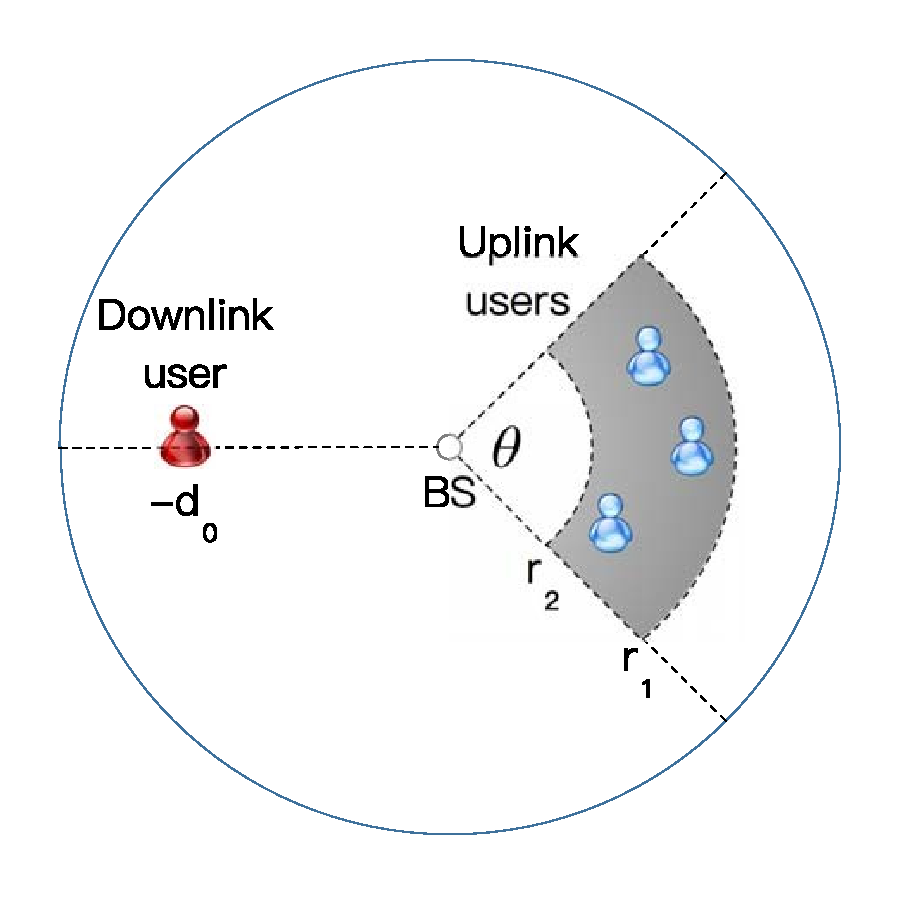
\includegraphics[width=1\linewidth]{images/fig1.pdf}
			\caption{1}
			%\label{fig:fig1}
		\end{figure}
		
		\column{.65\textwidth}
		\begin{enumerate}
			\item Uplink sum rates 
			\begin{itemize}
				\item  NOMA, FD
			
				\begin{equation}
					R_{\text{FD}}^{\text{U}} = \log\left( 1 + \frac{\sum_{m = 1}^M P_{\text{U}}\left\vert h_m\right\vert^2}{ P_{\text{SI}}\left\vert h_{\text{SI}}\right\vert^2 + 1} \right),
				\end{equation}
				\item NOMA, HD
				\begin{equation}
					R_{\text{HD}}^{\text{U}} = \frac{1}{2}\log\left( 1 + \sum_{m=1}^MP_{\text{U}}\left\vert h_m \right\vert^2 \right),
				\end{equation}
				\item OMA,HD \begin{equation}
						R_{\text{OMA}}^{\text{U}} = \frac{1}{2M}\sum_{m=1}^M \log\left( 1+P_\text{U}\left\vert h_m\right\vert^2 \right).
					\end{equation}
			\end{itemize}
		\end{enumerate}
		\end{columns}
\end{frame}


\begin{frame}{\textbf{{\LARGE{P}}ERFORMANCE {\LARGE{A}}NALYSIS}}
	
	\begin{columns}
		\column{.35\textwidth}
		\begin{figure}
			\centering
			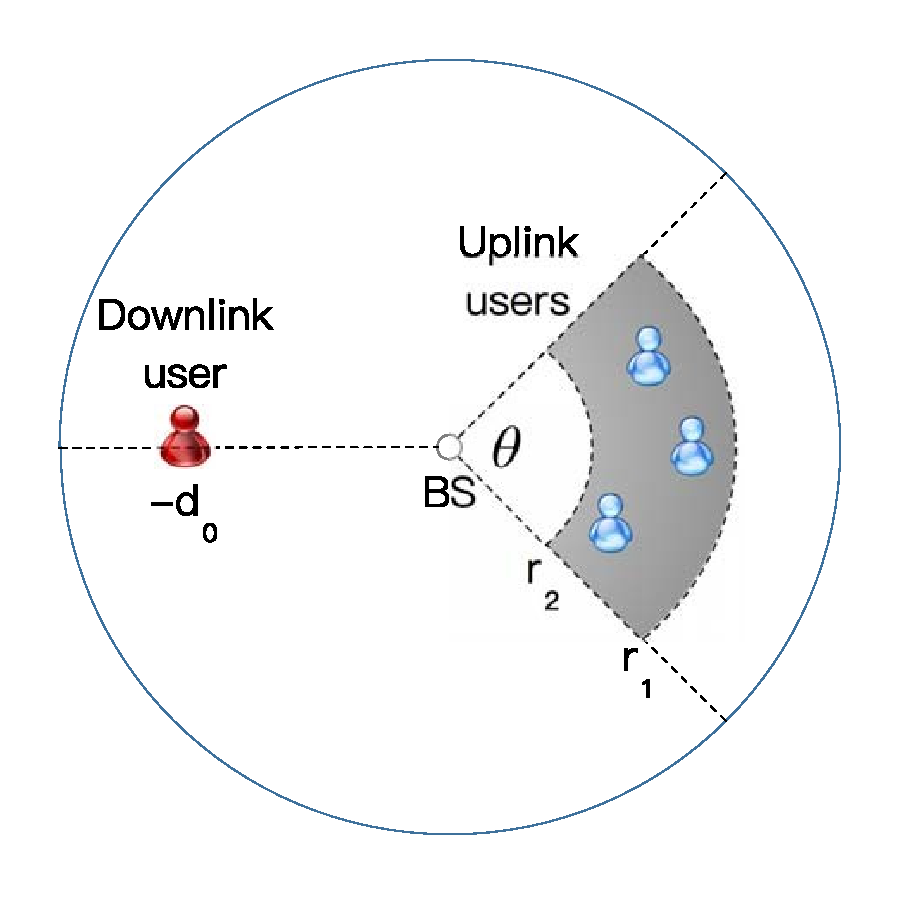
\includegraphics[width=1\linewidth]{images/fig1.pdf}
			\caption{1}
			%\label{fig:fig1}
		\end{figure}
		
		\column{.65\textwidth}
		\begin{enumerate}\setcounter{enumi}{1}
			\item Downlink sum rates 
			\begin{itemize}
				\item  NOMA, FD
				
				\begin{equation}
					R_{\text{FD}}^{\text{D}} = \log\left( 1 + \frac{P_{\text{BS}}\left\vert h_0\right\vert^2}{P_{\text{U}}\sum_{m=1}^M\left\vert g_m\right\vert^2+1}  \right),
				\end{equation}
				\item NOMA, HD
				\begin{equation}
					R_{\text{HD}}^{\text{D}} = \frac{1}{2}\log\left( 1 + P_{\text{BS}}\left\vert h_0 \right\vert^2 \right),
				\end{equation}
			\end{itemize}
		\end{enumerate}

		\begin{equation*}
		\mathrm{distance}(\text{DL user}, \text{UL user}) \geqslant d_0.
	\end{equation*}
	
	\end{columns}

\end{frame}

\begin{frame}
	\begin{figure}
		\centering
		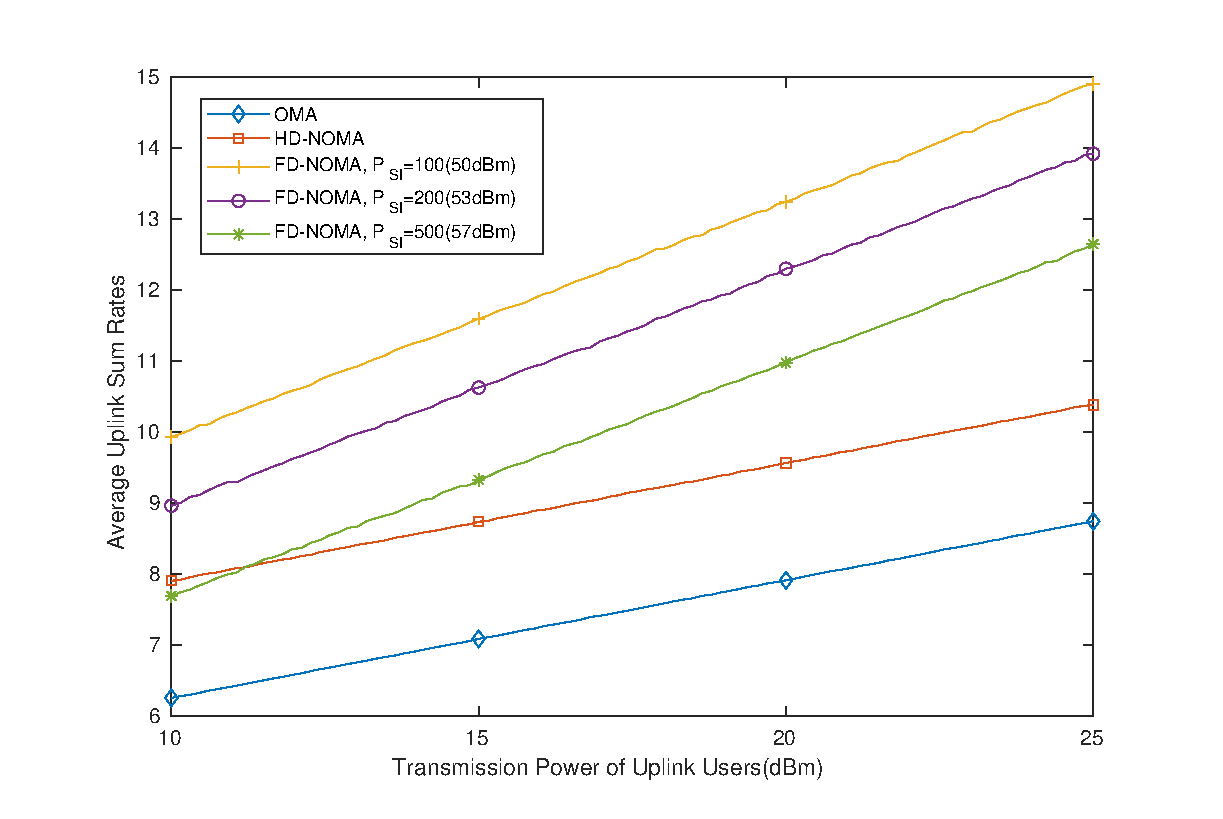
\includegraphics[width=0.7\linewidth]{images/2.eps}
		\caption{2.$\quad$ The uplink sum rates achieved by the three transmission schemes. Noise power of uplink transmission is $-61.5$dBm, $\alpha = 4$, $r_1 = 10$, $r_2 = 0$ and $\theta = \frac{\pi}{8}$.}
		\label{fig:fig2}
	\end{figure}
\end{frame}

\begin{frame}{\textbf{{\LARGE{M}}AIN {\LARGE{R}}ESULT}}
	\begin{enumerate}
		\item \(
			\mathrm{Pr}^{\text{U}} \triangleq \mathrm{Pr}\left( R_{\text{FD}}^{\text{U}}\leqslant R_{\text{HD}}^{\text{U}}\right)
		\): FD yields worse performance than HD (NOMA, uplink).\\
		\begin{equation}
			\mathrm{Pr}^{\text{U}}  = \mathrm{Pr}\left( \sum_{m=1}^M\left\vert h_m\right\vert^2 \leqslant\frac{P^2_{\text{SI}}y^2-1}{P_{\text{U}}} \right) \approx \cdots~\text{(Calculation)},
		\end{equation}
	其中$y\sim \mathcal{E}(1)$, $\left\vert h_m\right\vert^2$有分布函数: $F_{\left\vert h_m\right\vert^2}(t) = 1- \frac{2}{r_1^2-r_2^2}\int_{r^2}^{r_1}\mathrm{e}^{-r^\alpha t}r\mathrm{d}r$.
		\item \(
		\mathrm{Pr}^{\text{D}} \triangleq \mathrm{Pr}\left( R_{\text{FD}}^{\text{D}}\leqslant R_{\text{HD}}^{\text{D}}\right)
		\): FD yields worse performance than HD (NOMA, downlink).\\
			\begin{equation}
				\mathrm{Pr}^{\text{D}} = \mathrm{Pr}\left( \left\vert h_0\right\vert^2\leqslant \frac{P_{\text{U}}^2z^2 - 1}{P_{\text{BS}}}  \right)\approx\cdots~\text{(Calculation)}.
			\end{equation}
		其中$z = \sum_{m=1}^M\left\vert g_m\right\vert^2$
	\end{enumerate}
\end{frame}
	
\begin{frame}
	\begin{figure}
		\centering
		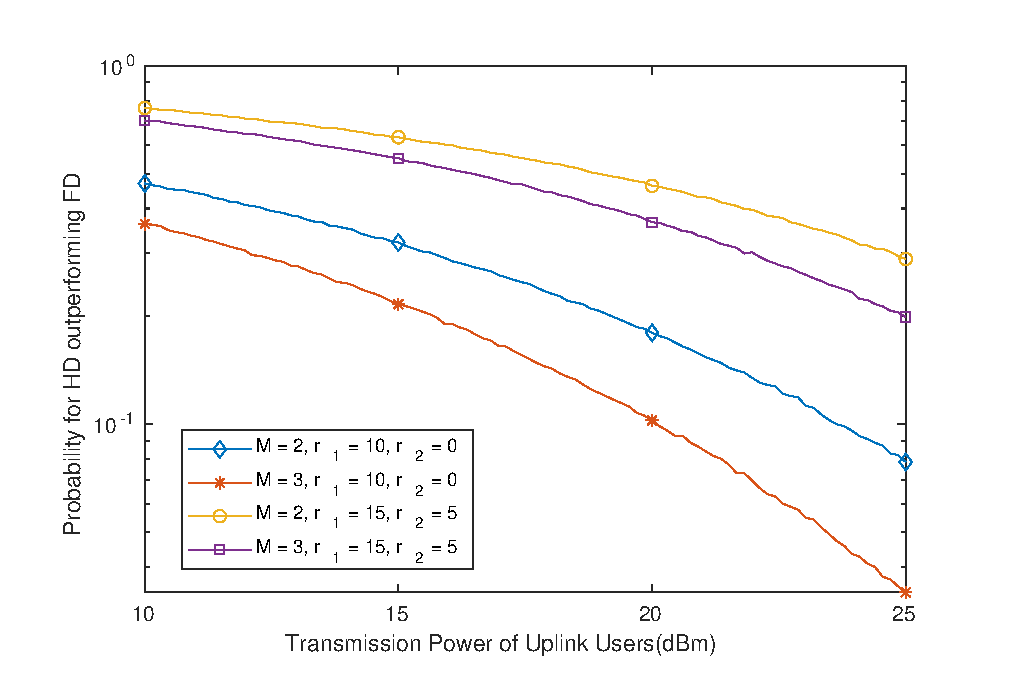
\includegraphics[width=0.7\linewidth]{images/3.eps}
		\caption{3.$\quad$ The probability $P(R_{\text{FD}}^{\text{U}}\leqslant R_{\text{HD}}^{\text{U}})$ versus the user transmission power. $\alpha = 4$, $\theta = \frac{\pi}{8}$, and $P_{\text{SI}} = 200(53dBm)$.}
		\label{fig:fig3}
	\end{figure}
\end{frame}

\begin{frame}
		\begin{figure}
			\centering
			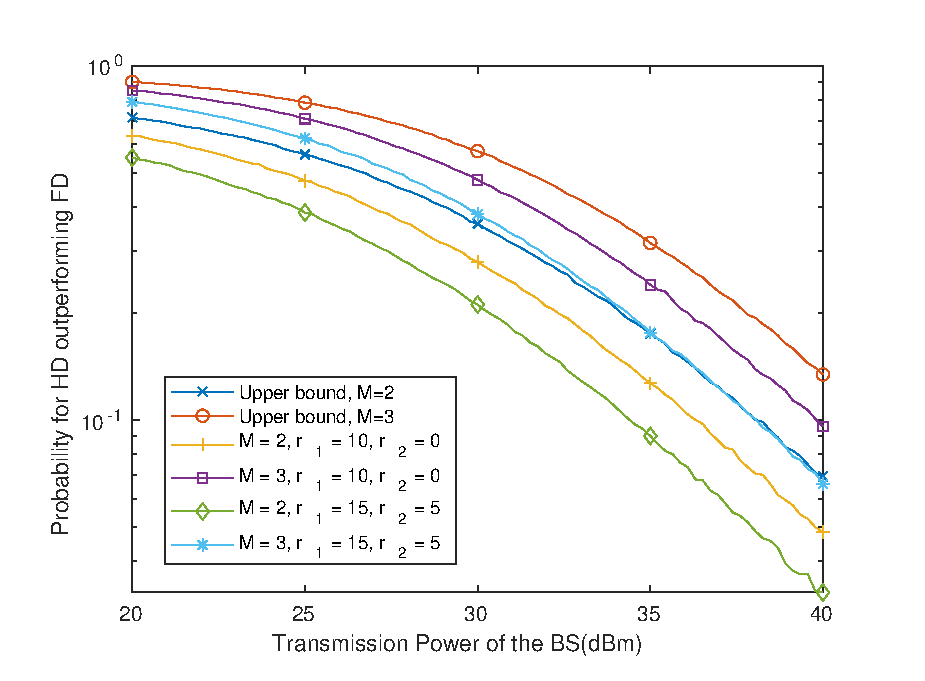
\includegraphics[width=0.65\linewidth]{images/4.eps}
			\caption{4.$\quad$ The probability $P(R_{\text{FD}}^{\text{D}}\leqslant R_{\text{HD}}^{\text{D}})$ versus the BS transmission power. $\alpha = 4$, $\theta = \frac{\pi}{8}$, and $P_{\text{U}} = 20\text{dBm}$, $d_0 = 100$.}
			\label{fig:fig4}
		\end{figure}
\end{frame}
	
\begin{frame}{\textbf{{\LARGE{M}}ATHEMATICS}}
	Chebyshev-Gauss quadrature(approximation):
	\begin{equation}
		\int_{-1}^{1}f(x)\mathrm{d}x \approx \sum_{j=1}^n \frac{\pi}{n} f(x_j)\sqrt{1-x_j^2},\, x_j = \cos(\frac{2j - 1}{2n}\pi).
	\end{equation}	
	Probability Facts: \begin{itemize}
		\item $X\sim \mathcal{CN}(0,1) \Rightarrow\, \abs{X}^2\sim \mathcal{E}(1).$
		\item $X_1,\cdots X_n$与$X$独立同分布, 有公共的概率密度$f(x)$. 记$S_n = \sum_{j=1}^n X_j$的概率密度函数为$f_{S_n}(x)$. 若$f(x)$的Laplace变换$\psi(s) = \mathcal{L}(f(x)) = \mathbb{E}\mathrm{e}^{-sX}$收敛, 则$f_{S_n}(x)$的Laplace变换为$[\psi(s)]^n$.
		\item $X\sim$ Rayleigh, i.e. $f_X(x) = \frac{2x}{\Omega}\mathrm{e}^{-\frac{x^2}{\Omega}}\bm{1}_{(x\geqslant 0)}$, $\Omega = \mathbb{E}X^2$ $\Rightarrow$ $Y=X^2\sim \mathcal{E}(1/\Omega)$.
	\end{itemize}
	
	
\end{frame}

\begin{frame}{\textbf{{\LARGE{M}}ATHEMATICS}}
	Integral:
	\begin{equation}
		\begin{split}
		\int_0^{\infty}x^k \mathrm{e}^{-a x^2-b x}\mathrm{d}x &= \frac{1}{2} a^{-\frac{k}{2}-1} \bigg(\sqrt{a} \Gamma \left(\frac{k+1}{2}\right)
			\, _1F_1\left(\frac{k+1}{2};\frac{1}{2};\frac{b^2}{4 a}\right) \\
			&\,\,\,\,\,\,-b \Gamma
			\left(\frac{k}{2}+1\right) \, _1F_1\left(\frac{k}{2}+1;\frac{3}{2};\frac{b^2}{4
				a}\right)\bigg)\\
			&= \Gamma(k+1)\mathrm{e}^{b^2/8a}(2a)^{-(k+1)/2}D_{-k-1}(b/\sqrt{2a}).
			\end{split}
	\end{equation}
	其中, $\,_1F_1$表示 Kummer's confluent hypergeometric function: \begin{equation}
		\,_1F_1(a;b;z)\coloneqq \sum_{n=0}^{\infty} \frac{(a)_n}{(b)_n}\frac{z^n}{n!},\, (q)_n = \begin{cases}
			1,&n = 0,\\
			q(q+1)\cdots(q+n-1), &n>0.
		\end{cases}
	\end{equation}
\end{frame}

\begin{frame}{\textbf{{\LARGE{M}}ATHEMATICS}}
	$D_{\nu}(\cdot)$是Parabolic cylinder functions(Whittaker \& Watson):
	\begin{equation}
		\begin{split}
		D_{\nu}(z) &= \frac{1}{\sqrt{\pi}}2^{\nu/2}\mathrm{e}^{-z^2/4}\bigg( \cos(\frac{\pi}{2}\nu)\Gamma\Big(\frac{\nu+1}{2}\Big)\,_1F_1\Big(-\frac{\nu}{2};\frac{1}{2};\frac{z^2}{2}\Big)\\
		&+\sqrt{2}z\sin(\frac{\pi}{2}\nu)\Gamma\Big(\frac{\nu}{2}+1\Big)\,_1F_1\Big(\frac{1}{2} - \frac{\nu}{2};\frac{3}{2};\frac{z^2}{2}\Big)\bigg),~~\nu > 0.
		\end{split}
	\end{equation}
\end{frame}

\begin{frame}{使用MMA软件检查计算结果:}
    \begin{figure}
		\centering
		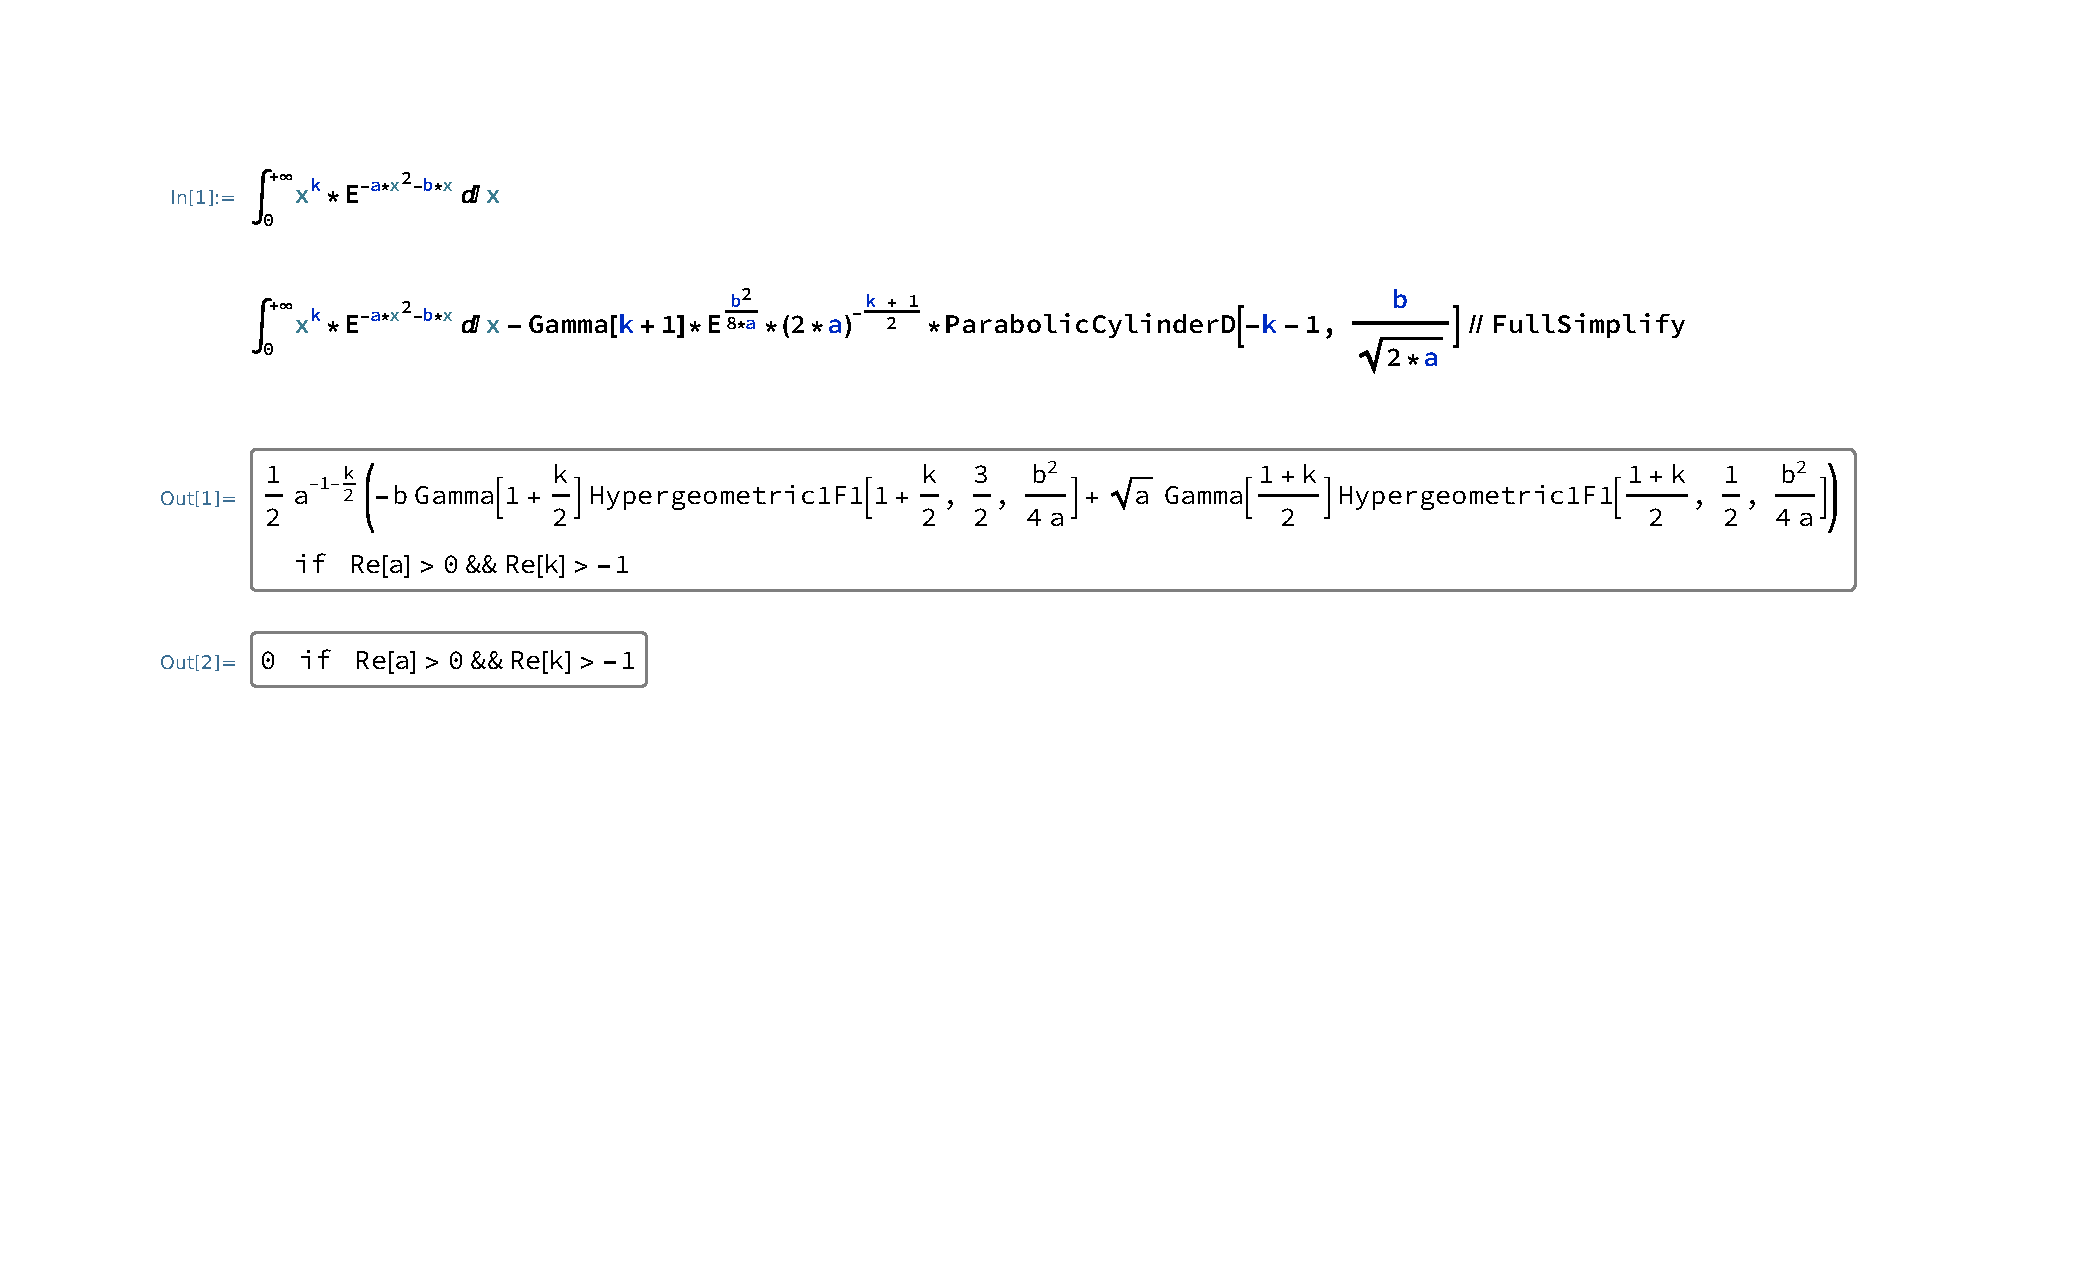
\includegraphics[width=1.0\linewidth, trim=70 0 100 0,clip]{images/print.pdf}
	\end{figure}
\end{frame}
%\section{概率空间}
    
    \frame{\sectionpage}
    
    \begin{frame}{概率空间}
        \begin{itemize}
        	\item 试验与事件
        	\item 古典型概率、几何型概率
        	\item 概率空间
        	\item 概率的性质
        	\item 条件概率和乘法公式
        	\item 事件的独立性
        	\item 全概率公式和Bayes公式
        	\item 概率空间的例子
        	\item Borel-Cantelli引理
        \end{itemize}
    \end{frame}
    

	\begin{frame}
		\Large\alert{
			在此,请同学们相信我们所提到的构造集合的方法都不会导致悖论.集合论中涉及数学基础的那些深层问题,也不会自己跳出来颠覆人们所发展的概率论方法.
		}
		\\ \hspace*{\fill} \\%空行
		在正式开始学习概率论之前,让我们先复习一下集合论的一些简单知识.这些知识构成了概率论语言的基础.我们假定大家对于朴素的集合论已经具有了一定的了解,因此只将这些介绍蜻蜓点水式地简单回顾.
	\end{frame}

	\begin{frame}{Sets}
		\begin{block}{\textbf{Definition}}
			\begin{itemize}
				\item \alert{集合}就是一些东西的总体.
				\item 总体中的东西称为这个集合的\alert{元素}
				\item 元素$\omega$是集合$A$的一个元素,称作元素$\omega$属于集合$A$,记作$\omega\in A$或者$A\ni\omega$.
				\item 在一个数学问题中,常有这样一个集合$\Omega$,使得问题中出现的所有集合都是它的子集.这个集合$\Omega$常被称为(这个问题的)\alert{空间}.
			\end{itemize}	
		\end{block}
	\end{frame}











% \section*{Acknowledgments}


\section{}
\begin{frame}{}
\centering
\Huge\bfseries
\textcolor{orange}{THANKS}
\end{frame}
\end{document}
